% !TeX root = ../analisi_2.tex

\section{Forme differenziali lineari}

\subsection{Definizione di forma differenziale lineare}

Sia $F : A \subseteq \mathbb{R}^3 \to \mathbb{R}^3$, $A$ aperto, $A \neq \emptyset$, $F$ continua:
\[
\underbrace{F(x, y, z)}_{\text{campo vett.}} = (F_1(x, y, z), F_2(x, y, z), F_3(x, y, z)) \qquad \text{($F$ continuo $\iff F_1, F_2, F_3$ continue)}
\]
Sia $\gamma(t)$ la curva in $\mathbb{R}^3$ che individua la ``traiettoria'' di $(x, y, z)$ in $t$:
\[
\gamma : [a, b] \to (x(t), y(t), z(t)) \in A \subseteq \mathbb{R}^3
\]
Il lavoro elementare è:
\[
dL := \langle \vec{F}, \underbrace{d\vec{r}}_{\substack{\text{spostamento elementare} \\ d\vec{r} = (dx, dy, dz) = dx\,\hat{\imath} + dy\,\hat{\jmath} + dz\,\hat{k}}} \rangle = F_1(x, y, z)\, dx + F_2(x, y, z)\, dy + F_3(x, y, z)\, dz
\]
\[
L = \int_\gamma dL = \int_a^b \left( F_1(\gamma(t))\, x'(t) + F_2(\gamma(t))\, y'(t) + F_3(\gamma(t))\, z'(t) \right) dt
\]
\pencilnote{Ricordando: $f \in C^1 \to \nabla f$. Confronto: $df(x_0, y_0, z_0) = f_x(x_0, y_0, z_0)\, dx + f_y(x_0, y_0, z_0)\, dy + f_z(x_0, y_0, z_0)\, dz =$ differenziale.}

\begin{definition}[Forma differenziale lineare]
Sia $F$ un campo vettoriale continuo, $F : A \subseteq \mathbb{R}^n \to \mathbb{R}^n$, $A \neq \emptyset$, aperto.

Si chiama \underline{forma differenziale lineare} con coefficienti $F_i$, $i = 1, \dots, n$ la seguente:
\[
\omega = F_1(x_1, \dots, x_n)\, dx_1 + F_2(x_1, \dots, x_n)\, dx_2 + \dots + F_n(x_1, \dots, x_n)\, dx_n = F_1(x)\, dx_1 + \dots + F_n(x)\, dx_n
\]
\pencilnote{È un funzionale lineare (è una funzione che ad un punto $x$ associa una combinazione lineare delle proiezioni $dx_i$).}

In particolare:
\begin{itemize}
    \item $n = 3 \implies \omega = F_1\, dx + F_2\, dy + F_3\, dz$
    \item $n = 2 \implies \omega = a(x, y)\, dx + b(x, y)\, dy$
\end{itemize}
\end{definition}

\subsection{Integrale di linea di una forma differenziale}

\begin{definition}[Integrale di linea e circuitazione]
Si definisce \underline{integrale di linea} di $\omega$ lungo una curva $\gamma : [a, b] \to A \subseteq \mathbb{R}^n$, $\gamma$ regolare, il seguente:
\[
\boxed{\int_\gamma \omega := \int_a^b \left( F_1(\gamma(t))\, x_1'(t) + F_2(\gamma(t))\, x_2'(t) + \dots + F_n(\gamma(t))\, x_n'(t) \right) dt}
\]
\pencilnote{(EXE: $\displaystyle\int_\gamma \underbrace{y}_{F_1}\, dx$)}

Se $\gamma$ è una curva \underline{chiusa}, il seg.:
\[
\oint_\gamma \omega \quad \text{si chiama \underline{circuitazione}}
\]
\end{definition}

Considero $\dfrac{|\gamma'(t)|}{|\gamma'(t)|} \cdot (\text{integrando})$. Quindi:
\[
\int_a^b \left( F_1(\gamma(t)) \frac{x_1'(t)}{|\gamma'(t)|} + \dots + F_n(\gamma(t)) \frac{x_n'(t)}{|\gamma'(t)|} \right) |\gamma'(t)|\, dt = \int_\gamma \langle F, T_\gamma \rangle\, ds
\]
\pencilnote{È un integrale curvilineo ($\displaystyle\int_\gamma f\, ds$).}
\[
\implies \int_\gamma \omega \text{ dip. dal verso} \implies
\begin{cases}
\gamma \stackrel{\circ}{\sim} \varphi \implies \displaystyle\int_\gamma \omega = \int_\varphi \omega \\[8pt]
\displaystyle\int_{-\gamma} \omega = -\int_\gamma \omega
\end{cases}
\]

\begin{prop}[Proprietà]
\begin{enumerate}
    \item Linearità: $\displaystyle\int_\gamma (\alpha \omega_1 + \beta \omega_2) = \alpha \int_\gamma \omega_1 + \beta \int_\gamma \omega_2$
    \item $\displaystyle\int_{-\gamma} \omega = -\int_\gamma \omega$
    \item $\displaystyle\int_{\gamma_1 \cup \gamma_2} \omega = \int_{\gamma_1} \omega + \int_{\gamma_2} \omega$
\end{enumerate}
\end{prop}

\begin{esercizio}[EXE 1]
$\omega = x^2\, dx + yx\, dy$. Calcolare $\displaystyle\int_\gamma \omega$, dove $\gamma$ è l'arco di parabola $y = x^2$, $x \in [-1, 1]$ nel senso delle $t$ cresc.
\end{esercizio}

\begin{esercizio}[EXE 2]
Calcolare $\displaystyle\int_\gamma \frac{xy}{\sqrt{x^2 + y^2}}\, dx - \frac{y}{\sqrt{x^2 + y^2}}\, dy$, con $\gamma = +\partial C$ e $C = \{ 1 \le x^2 + y^2 \le 4 \}$.
\end{esercizio}

\subsection{Forme differenziali esatte e primitive}

\begin{oss}
Se $f \in C^1$: $\omega = df$, $F = \nabla f$ \pencilnote{(posso vedere tutte le forme diff. come aventi coeff. $F_i$ che sono comp. di un gradiente)}.

Per $n = 1 \implies \omega = F(x)\, dx$.
\end{oss}

\begin{definition}[Primitiva]
Sia $\omega = F_1\, dx_1 + \dots + F_n\, dx_n$ definita in $A \subseteq \mathbb{R}^n$, $A \neq \emptyset$ e aperto.

Sia $g \in C^1(A)$; $g$ si dice \underline{primitiva} di $\omega$ se $F = \nabla g$, ovvero
\[
\begin{cases}
F_1 = g_{x_1} \\
\ \vdots \\
F_n = g_{x_n}
\end{cases}
\qquad \text{ovvero se } \omega = dg
\]
\end{definition}

\begin{prop}
Se $A$ è connesso, allora tutte le primitive di $\omega$, se $\exists$, differiscono per una costante.
\end{prop}

\begin{proof}
(vedi Analisi 1, per exe)
\end{proof}

\begin{esercizio}[EXE]
$\omega = 3x^2\, dx - xy\, dy$. Cerchiamo $\exists f \in C^1(\mathbb{R}^2) : f_x = 3x^2, \ f_y = -xy$:
\[
f(x, y) = \int 3x^2\, dx + c(y) = x^3 + c(y)
\]
Derivo in $y$:
\[
\frac{\partial}{\partial y} f(x, y) = c'(y) = -xy \to \text{non è possibile (dovrebbe solo dip. da $y$)}
\]
\end{esercizio}

\begin{definition}[Forma differenziale esatta]
Una forma differenziale $\omega$ si dice \underline{esatta} se $\exists$ una primitiva.
\end{definition}

\begin{oss}
\begin{center}
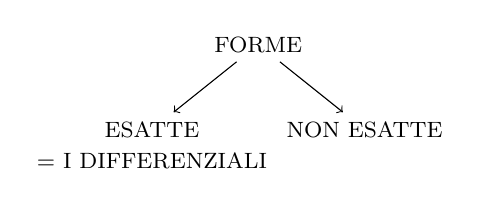
\begin{tikzpicture}[scale=0.9]
    \node (F) at (0,1.2) {\footnotesize FORME};
    \node (E) at (-1.5,0) {\footnotesize ESATTE};
    \node (NE) at (1.5,0) {\footnotesize NON ESATTE};
    \node at (-1.5,-0.45) {\footnotesize $=$ I DIFFERENZIALI};
    \draw[->] (F) -- (E);
    \draw[->] (F) -- (NE);
\end{tikzpicture}
\end{center}
\end{oss}

\begin{theorem}[Integra. forme esatte]
Sia $\omega = F_1\, dx_1 + \dots + F_n\, dx_n$ definita in $A \subseteq \mathbb{R}^n$, aperto, $A \neq \emptyset$.

Sia $\gamma$ una curva regolare a tratti con sostegno contenuto in $A$ e siano $P = \gamma(a)$ e $Q = \gamma(b)$ i suoi punti iniziale e finale rispettivamente.

Se $\omega$ è esatta, detta $f$ una primitiva allora:
\[
\boxed{\int_\gamma \omega = f(Q) - f(P) = f(\gamma(b)) - f(\gamma(a))}
\]
\begin{center}
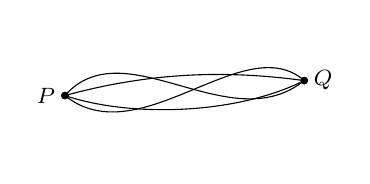
\begin{tikzpicture}[scale=0.95]
    \coordinate (P) at (0,0);
    \coordinate (Q) at (3.2,0.2);
    \draw (P) .. controls (0.8,0.9) and (2.2,-0.6) .. (Q);
    \draw (P) .. controls (1.0,-0.8) and (2.4,0.9) .. (Q);
    \draw (P) .. controls (1.1,0.3) and (2.1,0.35) .. (Q);
    \draw (P) .. controls (0.9,-0.3) and (2.3,-0.25) .. (Q);
    \fill (P) circle (1.5pt) node[left] {\footnotesize $P$};
    \fill (Q) circle (1.5pt) node[right] {\footnotesize $Q$};
\end{tikzpicture}
\end{center}
\end{theorem}

\begin{esercizio}[EXE 2 della scorsa]
Calcolare
\[
\int_\gamma \underbrace{\frac{xy}{\sqrt{x^2 + y^2}}\, dx - \frac{y}{\sqrt{x^2 + y^2}}\, dy}_{\omega}
\]
con $\gamma = +\partial E$ ed $E = \{ 1 \le x^2 + y^2 \le 4 \}$.
\[
F = \left( \frac{xy}{\sqrt{x^2 + y^2}}, \ -\frac{y}{\sqrt{x^2 + y^2}} \right)
\]
\begin{center}
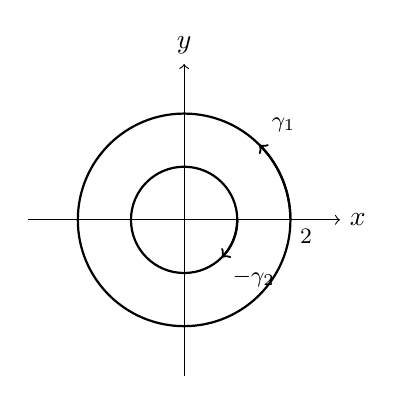
\begin{tikzpicture}[scale=0.9]
    \draw[->] (-2.2,0) -- (2.2,0) node[right] {$x$};
    \draw[->] (0,-2.2) -- (0,2.2) node[above] {$y$};
    \draw[thick] (0,0) circle (1.5);
    \draw[thick] (0,0) circle (0.75);
    \draw[->, thick] (1.5,0) arc (0:45:1.5);
    \draw[->, thick] (0.75,0) arc (0:-45:0.75);
    \node[below right] at (1.5,0) {\footnotesize $2$};
    \node[above right] at (1.1,1.1) {\footnotesize $\gamma_1$};
    \node[below right] at (0.55,-0.55) {\footnotesize $-\gamma_2$};
\end{tikzpicture}
\end{center}
\[
\gamma_1 = \begin{cases} x = 2 \cos t \\ y = 2 \sin t \end{cases} \quad t \in [0, 2\pi], \qquad \gamma_2 = \begin{cases} x = \cos t \\ y = \sin t \end{cases} \quad t \in [0, 2\pi]
\]
\[
\gamma = \gamma_1 \cup (-\gamma_2) \implies \oint_{\gamma_1} \omega - \oint_{\gamma_2} \omega = *
\]
\begin{align*}
\oint_{\gamma_1} \omega &= \int_0^{2\pi} \left( (-4) \cos t \sin^2 t - 2 \sin t \cos t \right) dt \\[4pt]
\oint_{\gamma_2} \omega &= \int_0^{2\pi} \left( -\cos t \sin^2 t - \sin t \cos t \right) dt
\end{align*}
\[
* = \int_0^{2\pi} \left[ (-4) \cos t \sin^2 t - 2 \sin t \cos t - \left( -\cos t \sin^2 t - \sin t \cos t \right) \right] dt = 0
\]
\end{esercizio}

\begin{theorem}[Integrale di forme esatte (già scritto)]
Sia $\omega = F_1\, dx_1 + \dots + F_n\, dx_n$, $F_i : A \subseteq \mathbb{R}^n \to \mathbb{R}$, $A \neq \emptyset$, $A$ aperto.

Assumiamo $\omega$ esatta e sia $f$ una primitiva.

Se $\gamma : [a, b] \to \mathbb{R}^n$ è una curva regolare a tratti con $\gamma([a, b]) \subseteq A$ allora
\[
\boxed{\int_\gamma \omega = f(\gamma(b)) - f(\gamma(a)) = f(Q) - f(P)}
\]
\end{theorem}

\begin{proof}
Sia $\gamma(t) = (x_1(t), \dots, x_n(t))$, $t \in [a, b]$ regolare.

\pencilnote{(Per curve reg. a tratti: applico sui tratti e poi elido tipo $f(P_2) - f(P_1)$)}
\begin{center}
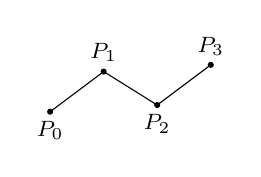
\begin{tikzpicture}[scale=0.85]
    \coordinate (P0) at (0,0);
    \coordinate (P1) at (0.8,0.6);
    \coordinate (P2) at (1.6,0.1);
    \coordinate (P3) at (2.4,0.7);
    \draw (P0) -- (P1) -- (P2) -- (P3);
    \fill (P0) circle (1.3pt) node[below] {\footnotesize $P_0$};
    \fill (P1) circle (1.3pt) node[above] {\footnotesize $P_1$};
    \fill (P2) circle (1.3pt) node[below] {\footnotesize $P_2$};
    \fill (P3) circle (1.3pt) node[above] {\footnotesize $P_3$};
\end{tikzpicture}
\end{center}

\[
\int_\gamma \omega \underset{\text{def}}{=} \int_a^b \left( F_1(\gamma(t))\, x_1'(t) + F_2(\gamma(t))\, x_2'(t) + \dots + F_n(\gamma(t))\, x_n'(t) \right) dt =
\]
$\omega$ esatta $\implies F_1(\gamma(t)) = f_{x_1}(\gamma(t)), \ \dots, \ F_n(\gamma(t)) = f_{x_n}(\gamma(t)) \implies$
\[
= \int_a^b \langle \nabla f(\gamma(t)), \gamma'(t) \rangle \, dt \overset{?}{=} \int_a^b \frac{d}{dt} G(t) \, dt = *
\]
Pongo $G(t) = f(\gamma(t))$. \pencilnote{Teo di der. funz. comp. ($f$ è diff.?)}

Essendo $f$ una primitiva, per def. essa è $C^1$, quindi per il teo del diff. totale è diff. $\implies * = G(b) - G(a)$.
\end{proof}

\begin{esercizio}[EXE]
\[
\omega = \frac{-y}{x^2 + y^2}\, dx + \frac{x}{x^2 + y^2}\, dy
\]
\[
F = \left( \frac{-y}{x^2 + y^2}, \ \frac{x}{x^2 + y^2} \right) \qquad \text{è ``conservativo''?}
\]
Considero $\gamma$:
\begin{center}
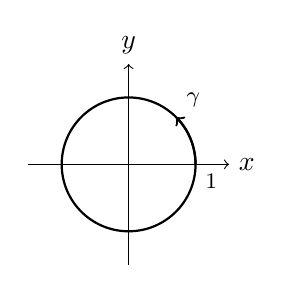
\begin{tikzpicture}[scale=0.85]
    \draw[->] (-1.5,0) -- (1.5,0) node[right] {$x$};
    \draw[->] (0,-1.5) -- (0,1.5) node[above] {$y$};
    \draw[thick] (0,0) circle (1.0);
    \draw[->, thick] (1.0,0) arc (0:45:1.0);
    \node[below right] at (1.0,0) {\footnotesize $1$};
    \node[above right] at (0.72,0.72) {\footnotesize $\gamma$};
\end{tikzpicture}
\end{center}
\[
\oint_\gamma \omega = \int_0^{2\pi} \left( \sin^2 t + \cos^2 t \right) dt = 2\pi \neq 0 \implies \omega \text{ non è esatta.}
\]
\end{esercizio}

\subsection{Teorema di caratterizzazione delle forme esatte}

\begin{theorem}[Teorema di caratterizzazione delle forme esatte]
\begin{itemize}
    \item Sia $A \subseteq \mathbb{R}^n$, $A \neq \emptyset$, $A$ aperto e \underline{connesso}.
    \item Sia $\omega = F_1\, dx_1 + \dots + F_n\, dx_n$ def. su $A$.
\end{itemize}
Allora sono equivalenti i seguenti:
\begin{enumerate}
    \item $\omega$ è esatta
    \item $\forall$ curva $\gamma$ regolare a tratti chiusa $\displaystyle\oint_\gamma \omega = 0$
    \item $\forall \gamma_1, \gamma_2$ curve regolari a tratti con stessi estremi e verso di percorrenza risulta $\displaystyle\int_{\gamma_1} \omega = \int_{\gamma_2} \omega$.
\end{enumerate}
\end{theorem}

\begin{proof}
$1) \overset{\text{a}}{\implies} 2) \overset{\text{b}}{\implies} 3) \overset{\text{c}}{\implies} 1)$

\begin{itemize}
    \item \textbf{a)} Ovvia dal teo prec.

    \item \textbf{b)} Hp: $\displaystyle\oint_\gamma \omega = 0 \implies \int_{\gamma_1} \omega = \int_{\gamma_2} \omega$ $\forall \gamma_1, \gamma_2$ hanno stessi pti iniziali e finali (Th).

    \begin{center}
    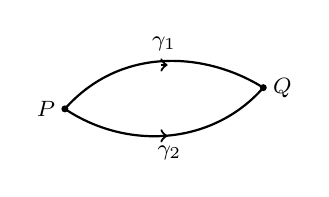
\begin{tikzpicture}[scale=0.9]
        \coordinate (P) at (0,0);
        \coordinate (Q) at (2.8,0.3);
        \draw[thick] (P) .. controls (0.8,0.9) and (2.0,0.8) .. (Q) node[midway, above] {\footnotesize $\gamma_1$};
        \draw[->, thick] (1.35,0.62) -- (1.45,0.62);
        \draw[thick] (P) .. controls (0.9,-0.6) and (2.1,-0.5) .. (Q) node[midway, below] {\footnotesize $\gamma_2$};
        \draw[->, thick] (1.35,-0.38) -- (1.45,-0.38);
        \fill (P) circle (1.4pt) node[left] {\footnotesize $P$};
        \fill (Q) circle (1.4pt) node[right] {\footnotesize $Q$};
    \end{tikzpicture}
    \end{center}
    \[
    \implies \gamma = \gamma_1 \cup (-\gamma_2) \implies \oint_{\gamma = \gamma_1 \cup (-\gamma_2)} \omega = 0 \quad \text{per Hp}
    \]
    \[
    \implies \int_{\gamma_1} \omega + \int_{-\gamma_2} \omega = 0 \implies \int_{\gamma_1} \omega = \int_{\gamma_2} \omega \quad \text{è la tesi.}
    \]

    \item \textbf{c)} (Hp): $\displaystyle\int_{\gamma_1} \omega = \int_{\gamma_2} \omega$ $\forall \gamma_1, \gamma_2$ stessi pti iniziali e finali $\implies \omega$ esatta (Th).

    Considero $x_0 \in A$ e poiché è aperto $\exists x \in A, \ x \neq x_0$.

    $A$ poiché è connesso ed è aperto $\implies$ è connesso per poligonali \pencilnote{(la poligonale è una curva)}.
    \[
    \boxed{f(x) = \int_{\gamma_{[x_0, x]}} \omega} \qquad \forall x \in A \qquad \text{\pencilnote{($x_0$ fisso, $x$ ``mobile'')}}
    \]
    Mostriamo che $\nabla f = F$ \pencilnote{($F$ è il campo dei coefficienti di $\omega$)}.

    Mostriamo la $f_{x_1} = F_1$, per le altre si rag. allo stesso modo:
    \[
    f_{x_1}(x) = \lim_{h \to 0} \frac{f(x + h e_1) - f(x)}{h} = \lim_{h \to 0} \frac{\displaystyle\int_{\gamma_{[x_0, x + h e_1]}} \omega - \int_{\gamma_{[x_0, x]}} \omega}{h} =
    \]
    \begin{center}
    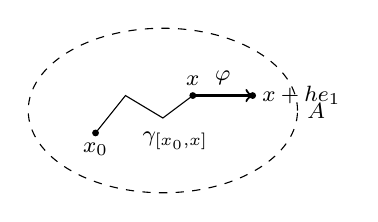
\begin{tikzpicture}[scale=0.95]
        \draw[dashed] (1.5,1.0) ellipse (1.8 and 1.1);
        \node[right] at (3.3,1.0) {\footnotesize $A$};
        \coordinate (X0) at (0.6,0.7);
        \coordinate (A1) at (1.0,1.2);
        \coordinate (A2) at (1.5,0.9);
        \coordinate (X) at (1.9,1.2);
        \coordinate (XH) at (2.7,1.2);
        \draw (X0) -- (A1) -- (A2) -- (X);
        \draw[thick, ->] (X) -- (XH) node[midway, above] {\footnotesize $\varphi$};
        \fill (X0) circle (1.3pt) node[below] {\footnotesize $x_0$};
        \fill (X) circle (1.3pt) node[above] {\footnotesize $x$};
        \fill (XH) circle (1.3pt) node[right] {\footnotesize $x + h e_1$};
        \node[below right] at (1.1,0.85) {\footnotesize $\gamma_{[x_0, x]}$};
    \end{tikzpicture}
    \end{center}
    Se scelgo $\gamma_{[x_0, x + h e_1]} = \gamma_{[x_0, x]} \cup \varphi$ con $\varphi$ segmento che congiunge $x$ con $x + h e_1$, allora si ha:

    $\implies$ uso additività nel limite $\implies$ rimane solo:
    \[
    \lim_{h \to 0} \frac{1}{h} \left[ \int_\varphi \omega \right] \implies \text{parametrizzo } \varphi
    \]
    Ma sia $\varphi = \begin{cases} x_1 = x_1 + t \\ x_2 = x_2 \\ \ \vdots \\ x_n = x_n \end{cases} \quad t \in [0, h]$ \pencilnote{($x_2' = x_3' = \dots = x_n' = 0$)}:
    \[
    \text{Il lim} = \lim_{h \to 0} \frac{1}{h} \int_0^h F_1(x_1 + t, x_2, \dots, x_n) \cdot \underbrace{x_1'}_{1} \, dt \implies \text{teo della media integrale}
    \]
    \pencilnote{oppure la vedo come derivata in $0$ rispetto a $t$.}

    Chiamo $G(x) = \displaystyle\int_0^x g(t) \, dt$, dove $F_1(x_1 + t, x_2, \dots, x_n)$ la vedo come una $g(t)$ $\implies$
    \[
    \lim_{h \to 0} \frac{1}{h} \int_0^h F_1(x_1 + t, \dots, x_n) \, dt = G'(0) \underset{\text{T.F.d.C.I.}}{=} F_1(x)
    \]
\end{itemize}
\end{proof}

\subsection{Forme differenziali chiuse e insiemi semplicemente connessi}

\begin{definition}[Forma differenziale chiusa]
Sia $\omega = F_1\, dx_1 + \dots + F_n\, dx_n$, con $F = (F_1, \dots, F_n) \in C^1(A)$, $A \subseteq \mathbb{R}^n$, $A \neq \emptyset$ e aperto.

$\omega$ si dice \underline{chiusa} (ovvero $F$ è \underline{irrotazionale}) se
\[
\frac{\partial F_i}{\partial x_j} = \frac{\partial F_j}{\partial x_i} \qquad \forall i, j = 1, \dots, n, \quad i \neq j
\]
\end{definition}

\begin{esercizio}[EXE]
$n = 2$: $\omega = a(x, y)\, dx + b(x, y)\, dy$:
\[
\frac{\partial a}{\partial y} = \frac{\partial b}{\partial x}
\]
\end{esercizio}

\begin{oss}
$\omega$ esatta $\overset{?}{\longleftrightarrow}$ $\omega$ chiusa. C'è una relazione?

Se $\omega$ esatta e il campo dei coeff. è $C^1(A) \implies \omega$ chiusa.
\end{oss}

\begin{prop}
\[
\omega \text{ esatta} \ + \ F \in C^1(A) \implies \omega \text{ chiusa.}
\]
\end{prop}

\begin{proof}
$\omega$ esatta $\implies F = \nabla f$, $f \in C^1(A)$:
\[
F_1 = f_{x_1}, \quad F_2 = f_{x_2}, \quad \dots, \quad F_n = f_{x_n}
\]
Ma $\omega$ per essere chiusa deve avere:
\[
\frac{\partial F_i}{\partial x_j} = \frac{\partial F_j}{\partial x_i} \quad \forall i \neq j \implies \frac{\partial f_{x_i}}{\partial x_j} = \frac{\partial f_{x_j}}{\partial x_i} \quad \forall i \neq j \iff f_{x_i x_j} \overset{?}{=} f_{x_j x_i} \quad \forall i \neq j \quad \text{(Th)}
\]
Ma $F \in C^1(A) \implies f \in C^2(A) \implies$ vale Schwarz.
\end{proof}

\begin{oss}
\underline{Non vale il viceversa}.
\end{oss}

\begin{esercizio}[EXE (Controesempio)]
\[
\omega = \underbrace{\frac{-y}{x^2 + y^2}}_{a(x, y)}\, dx + \underbrace{\frac{x}{x^2 + y^2}}_{b(x, y)}\, dy
\]
$A = \mathbb{R}^2 \setminus \{ (0, 0) \} \to$ questo dominio si dice \underline{bucato}. È connesso ma non convesso.

$\omega \in C^1(A)$. $\omega$ è chiusa? $\omega$ non è esatta perché $\displaystyle\oint \omega = 2\pi$.
\begin{align*}
\frac{\partial a}{\partial y} &= \frac{-(x^2 + y^2) + 2y^2}{(x^2 + y^2)^2} = \frac{y^2 - x^2}{(x^2 + y^2)^2} \\[4pt]
\frac{\partial b}{\partial x} &= \frac{x^2 + y^2 - 2x^2}{(x^2 + y^2)^2} = \frac{y^2 - x^2}{(x^2 + y^2)^2}
\end{align*}
Sono uguali $\implies$ è chiusa.
\end{esercizio}

\begin{definition}[Insieme semplicemente connesso ($\mathbb{R}^2$ non $\mathbb{R}^n$)]
Sia $A \subseteq \mathbb{R}^2$, $A \neq \emptyset$ e connesso.

$A$ si dice \underline{semplicemente connesso} se ogni curva chiusa e semplice con sostegno in $A$, racchiude un insieme che è tutto contenuto in $A$.
\end{definition}

\begin{theorem}[Rimandato]
Sia $\omega \in C^1(A)$, $A \subseteq \mathbb{R}^2$, $A$ sempl. connesso.

Se $\omega$ è chiusa, allora $\omega$ è esatta.
\end{theorem}

\begin{esercizio}[EXE]
\[
\omega = \left( y \log(1 - xy) + \frac{x}{x^2 + y^2 - 1} \right) dx + \left( x \log(1 - xy) + \frac{y}{x^2 + y^2 - 1} \right) dy
\]
e determinare una primitiva che si annulla nel punto $\left(0, \dfrac{1}{2}\right)$.

$\omega = \omega_1 + \omega_2$:
\begin{itemize}
    \item Studio $\omega_1$: $1 - xy > 0$.
    \begin{itemize}
        \item $\omega_1$ è def. in $A$ se. c.
        \item $\omega_1 \in C^1(A)$
        \item $\omega_1$ è chiusa? $*$
    \end{itemize}
    \begin{center}
    \begin{tikzpicture}[scale=0.85]
        \draw[->] (-1.8,0) -- (1.8,0) node[right] {$x$};
        \draw[->] (0,-1.8) -- (0,1.8) node[above] {$y$};
        \draw[thick, domain=0.35:1.6, smooth] plot (\x, {0.55/\x});
        \draw[thick, domain=-1.6:-0.35, smooth] plot (\x, {0.55/\x});
        \node[below right] at (0.8,-0.8) {\footnotesize dominio};
    \end{tikzpicture}
    \end{center}

    \item Studio $\omega_2$: $x^2 + y^2 \neq 1$.
    \begin{center}
    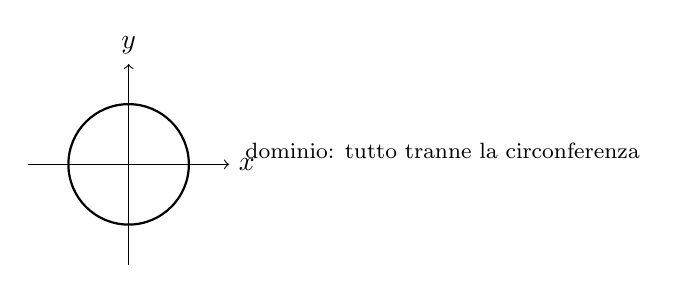
\begin{tikzpicture}[scale=0.85]
        \draw[->] (-1.5,0) -- (1.5,0) node[right] {$x$};
        \draw[->] (0,-1.5) -- (0,1.5) node[above] {$y$};
        \draw[thick] (0,0) circle (0.9);
        \node[right] at (1.6,0.2) {\footnotesize dominio: tutto tranne la circonferenza};
    \end{tikzpicture}
    \end{center}
\end{itemize}
$*$
\begin{align*}
\frac{\partial a}{\partial y} &= \log(1 - xy) - \frac{xy}{1 - xy} \\[4pt]
\frac{\partial b}{\partial x} &= \log(1 - xy) - \frac{yx}{1 - xy}
\end{align*}
Allora $\omega_1$ è esatta. Calcoliamo una primitiva $f_1(x, y)$:
\[
f_1(x, y) = \int a(x, y)\, dx = \int y \log(1 - xy)\, dx = -\int (-y) \log(1 - xy)\, dx = -\int \log(1 + t)\, dt
\]
\pencilnote{($-xy = t \implies -y\, dx = dt$)}
\[
= -\left[ (1 + t)\log(1 + t) - t \right] = \text{da vedere} = -(1 - xy)\log(1 - xy) - xy + c(y)
\]
\[
\frac{\partial f_1}{\partial y} = c'(y) - x + \frac{(1 - xy)}{(1 - xy)} \cdot (+x) - x \log(1 - xy) = b(x, y)
\]
\[
c'(y) + x \log(1 - xy) = x \log(1 - xy) \to c'(y) = 0 \to c(y) = \text{cost.}
\]
\[
f_1(x, y) = -\left[ xy + (1 - xy)\log(1 - xy) + c_1 \right]
\]

\begin{center}
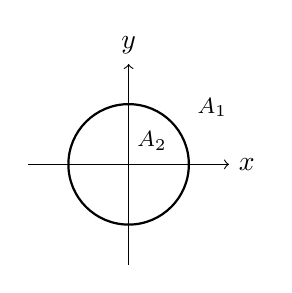
\begin{tikzpicture}[scale=0.85]
    \draw[->] (-1.5,0) -- (1.5,0) node[right] {$x$};
    \draw[->] (0,-1.5) -- (0,1.5) node[above] {$y$};
    \draw[thick] (0,0) circle (0.9);
    \node at (0.35,0.35) {\footnotesize $A_2$};
    \node at (1.25,0.85) {\footnotesize $A_1$};
\end{tikzpicture}
\end{center}
$A = A_1 \cup A_2$: $A$ è sconnesso ma $\omega_2$ è localmente esatta in $A_2$ (che è sempl. conn.).

Quindi in questo caso, in $\left(0, \dfrac{1}{2}\right)$ considero $\omega_2\big|_{A_2}$ è esatta.
\end{esercizio}

\begin{theorem}
Sia $\omega$ definita in $\mathbb{R}^2 \setminus \{ (0, 0) \}$ \pencilnote{(qualunque punto $(x_0, y_0)$)} e chiusa.

Se $\exists \gamma_0$ curva chiusa contenente $(0, 0)$ al suo interno, reg. a tratti e:
\[
\oint_{\gamma_0} \omega = 0 \qquad \text{\pencilnote{($\gamma_0$ ha sostegno in $\mathbb{R}^2 \setminus \{ (0, 0) \}$)}}
\]
allora $\omega$ è esatta.
\end{theorem}

\begin{proof}
Sia $\gamma$ un'altra curva chiusa regolare che contiene $(0, 0)$ al suo interno.

$\implies$ dimostro che $\displaystyle\oint_\gamma \omega = \oint_{\gamma_0} \omega$.

\begin{center}
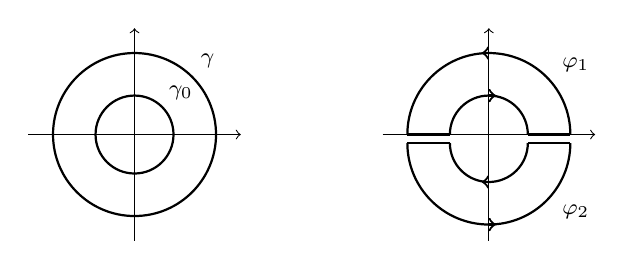
\begin{tikzpicture}[scale=0.9]
    % Schema 1
    \begin{scope}[shift={(-2.5,0)}]
        \draw[->] (-1.5,0) -- (1.5,0);
        \draw[->] (0,-1.5) -- (0,1.5);
        \draw[thick] (0,0) circle (0.55);
        \draw[thick] (0,0) circle (1.15);
        \node[above right] at (0.35,0.35) {\footnotesize $\gamma_0$};
        \node[above right] at (0.8,0.8) {\footnotesize $\gamma$};
    \end{scope}
    % Schema 2
    \begin{scope}[shift={(2.5,0)}]
        \draw[->] (-1.5,0) -- (1.5,0);
        \draw[->] (0,-1.5) -- (0,1.5);
        \draw[thick] (1.15,0) arc (0:180:1.15);
        \draw[thick] (-0.55,0) arc (180:0:0.55);
        \draw[thick] (-1.15,0) -- (-0.55,0);
        \draw[thick] (0.55,0) -- (1.15,0);
        \draw[->, thick] (0,1.15) -- (-0.1,1.15);
        \draw[->, thick] (0,0.55) -- (0.1,0.55);
        \draw[thick] (-1.15,-0.12) arc (180:360:1.15);
        \draw[thick] (0.55,-0.12) arc (360:180:0.55);
        \draw[thick] (-1.15,-0.12) -- (-0.55,-0.12);
        \draw[thick] (0.55,-0.12) -- (1.15,-0.12);
        \draw[->, thick] (0,-1.27) -- (0.1,-1.27);
        \draw[->, thick] (0,-0.67) -- (-0.1,-0.67);
        \node[above right] at (0.9,0.75) {\footnotesize $\varphi_1$};
        \node[below right] at (0.9,-0.85) {\footnotesize $\varphi_2$};
    \end{scope}
\end{tikzpicture}
\end{center}

$\omega$ è localmente esatta. Allora:
\[
\oint_{\varphi_1} \omega + \oint_{\varphi_2} \omega = 0
\]
\[
\oint_{\varphi_1} \omega + \oint_{\varphi_2} \omega = \int_{\varphi_1 \cup \varphi_2} \omega = \oint_\gamma \omega - \oint_{\gamma_0} \omega + \text{(contributo dei segmenti = nullo perché percorsi in 2 versi opposti)}
\]
\[
\implies 0 = \oint_{\varphi_1} \omega + \oint_{\varphi_2} \omega = \int_{\varphi_1 \cup \varphi_2} \omega = \oint_\gamma \omega - \oint_{\gamma_0} \omega = 0
\]
Se $\displaystyle\oint_{\gamma_0} \omega = 0 \implies \oint_\gamma \omega = 0$.
\end{proof}

\subsection{Forme radiali}

\begin{definition}[Forma radiale]
Una forma si dice \underline{radiale} se è in questa forma:
\[
\omega = \frac{x}{r} \varphi(r)\, dx + \frac{y}{r} \varphi(r)\, dy, \qquad r = \sqrt{x^2 + y^2}
\]
\pencilnote{($dr = \dfrac{x}{r}\, dx + \dfrac{y}{r}\, dy$)}

Posta $\Psi(r) = \displaystyle\int \varphi(r)\, dr \to f(x, y) = \Psi\left(\sqrt{x^2 + y^2}\right)$.
\end{definition}
